\documentclass[10pt, conference, compsocconf]{IEEEtran}
%\documentclass[preprint,10pt,nocopyrightspace]{sigplanconf}
%\documentclass[letterpaper, twocolumn, 10pt]{article}

\pdfpagewidth=8.5in
\pdfpageheight=11in

\usepackage{balance}
% comment out the following line when submitting
\def \oscardebug{}
%\def\inputGnumericTable{}
\newcommand{\subparagraph}{}

% rubber: paper letter

% $Id$

% natbib package in sigplanconf class file conflicts with cite package
%\usepackage{cite} 
\usepackage{paralist}
\usepackage{times}
\usepackage{framed}
%\usepackage[small,compact]{titlesec}
% XXX: This messes up margins
%\usepackage{geometry}
%\geometry{margin=1in}
\usepackage{graphicx}
\usepackage{subfig}
\usepackage{rotating}
\usepackage{fancybox}
%\usepackage{pstricks}
\usepackage{multirow}
\usepackage{listings}
\lstset{language=C}
\usepackage[hyphens]{url}
%\usepackage{endnotes}
\usepackage{comment}
\usepackage{alltt}
\usepackage{color}
%\usepackage{natbibspacing}

\usepackage[latin1]{inputenc}
%\usepackage[utf8]{inputenc} %Para configuraci�n de caracteres
%\usepackage[spanish]{babel} %Para configuraci�n de idioma

\usepackage{color}
\usepackage{array}
\usepackage{longtable}
\usepackage{calc}
\usepackage{multirow}
\usepackage{hhline}
\usepackage{ifthen}
\usepackage{lscape}
%\usepackage{graphicx}
\usepackage{wrapfig}
\usepackage{booktabs}
\usepackage{pbox}
\usepackage{ifthen}
\usepackage{wasysym}
\usepackage[sort]{natbib}

\renewcommand\settominwidth[3][\columnwidth]{%
   \settowidth{#2}{\begin{tabular}{@{}l@{}}#3\end{tabular}}%
   \ifthenelse{\lengthtest{#1<#2}}{\setlength{#2}{#1}}{}% extra brace group
}


\DeclareGraphicsExtensions{.pdf,.png,.jpg}

% Make list indentation tight
\setdefaultleftmargin{1em}{0em}{}{}{}{}

\begin{document}

%\singlespace
%% To make table entries readable
%\newcommand\T{\rule{0pt}{2.0ex}}
%\newcommand\B{\rule[-0.9ex]{0pt}{0pt}}

%% Eliminate widows and orphans if needed 
%% \clubpenalty 10000
%% \widowpenalty 10000
%% \def\topfraction{0.9}
%% \def\bottomfraction{0.9}
%% \def\textfraction{0.1}

% Squeeze space
%\renewcommand{\baselinestretch}{0.99}
%\addtolength{\belowcaptionskip}{-10pt}
%\addtolength{\abovecaptionskip}{-5pt}
%\newcommand{\tabpar}[2]{
%    \begin{center} \begin{tabular}{#1} #2 \end{tabular} \end{center}}

%% \newcommand{\by}[2]{\mbox{#1$\times$#2}}

%% \newcommand{\wunits}[2]{\mbox{#1\,#2}}
%% \newcommand{\um}{\mbox{$\mu$m}}
%% \newcommand{\xum}[1]{\wunits{#1}{\um}}
%% \newcommand{\xnm}[1]{\wunits{#1}{nm}}
%% \newcommand{\sig}[1]{${\tt #1}$}
%% \newcommand{\sigb}[1]{$\overline{{\tt #1}}$}

\ifx \oscardebug \undefined
\newcommand{\fixmedp}[1]{{}}
\else
\newcommand{\fixmedp}[1]{{\bf\textcolor{red}{ [ dP FIXME: #1 ]}}}
\fi

\ifx \oscardebug \undefined
\newcommand{\fixmebj}[1]{{}}
\else
\newcommand{\fixmebj}[1]{{\bf\textcolor{blue}{ [ bJ FIXME: #1 ]}}}
\fi

\ifx \oscardebug \undefined
\newcommand{\fixmebb}[1]{{}}
\else
\newcommand{\fixmebb}[1]{{\bf\textcolor{green}{ [ bB FIXME: #1 ]}}}
\fi

\ifx \oscardebug \undefined
\newcommand{\fixmedz}[1]{{}}
\else
\newcommand{\fixmedz}[1]{{\bf\textcolor{magenta}{ [ dZ FIXME: #1 ]}}}
\fi

\newcommand{\callout}[1]{\vspace{5pt}\noindent\fbox{\parbox{3.25in}{{#1}}}\vspace{5pt}}
\definecolor{darkgreen}{rgb}{0.000000,0.5,0.000000}
\newcommand{\change}[1]{{#1}}
\newcommand{\changebj}[1]{{\textcolor{magenta}{#1}}}

% MW adding. To compile without the red, either:
% (1) comment in the following line:
%\def\noeditingmarks{} % or
% (2) compile with a line like:
%    $ latex '\def\noeditingmarks{} \input osdi08
% Also, might be easier to convert your macros to this format. (I like
% having the comments in another color and also being able to turn them
% all off with one command.)
\begin{comment}
\newcommand{\textred}[1]{\textcolor{red}{#1}}
\ifx\noeditingmarks\undefined
    \newcommand{\pgwrapper}[2]{\textred{#1: #2}}
\else
    \newcommand{\pgwrapper}[2]{}
\fi
\newcommand{\mw}[1]{\pgwrapper{MW}{#1}}
\end{comment}
\newcommand*{\TitleFont}{%
	\usefont{\encodingdefault}{\rmdefault}{b}{n}%
	\fontsize{18}{20}%
	\selectfont}
\newcommand*{\SubtitleFont}{%
	\usefont{\encodingdefault}{\rmdefault}{b}{n}%
	\fontsize{14}{20}%
	\selectfont}

%\def\name#1{#1}%
%\def\defname#1#2{\expandafter\def\csname #1\endcsname{\name{#2}}\ignorespaces}%
%\thispagestyle{empty}

\title{\TitleFont PyNEMO 3: SE PERDIERON TODOS.\\ \SubtitleFont Una aplicaci�n \\con Algoritmos B�squeda informada y no informada}

%\authorinfo{names}{Stony Brook}{emails}
%\author{\IEEEauthorblockN{Dongli Zhang}
%\IEEEauthorblockA{Stony Brook University\\
%jeffersonamado
%}
%}
%\author{\IEEEauthorblockN{Authors Name/s per 1st Affiliation (Author)}
%\IEEEauthorblockA{line 1 (of Affiliation): dept. name of organization\\
%line 2: name of organization, acronyms acceptable\\
%line 3: City, Country\\
%line 4: Email: name@xyz.com}
%\and
%\IEEEauthorblockN{Authors Name/s per 2nd Affiliation (Author)}
%\IEEEauthorblockA{line 1 (of Affiliation): dept. name of organization\\
%line 2: name of organization, acronyms acceptable\\
%line 3: City, Country\\
%line 4: Email: name@xyz.com}
%\and
%\IEEEauthorblockN{Authors Name/s per 2nd Affiliation (Author)}
%\IEEEauthorblockA{line 1 (of Affiliation): dept. name of organization\\
%	line 2: name of organization, acronyms acceptable\\
%	line 3: City, Country\\
%	line 4: Email: name@xyz.com}
%}
%\author{\IEEEauthorblockN{Jefferson Amado Pe�a Torres}
%	\IEEEauthorblockA{Cod. 1329454\\jeffersonamado@correounivalle.edu.co\\
%		Universidad del Valle\\
%		Santiago de Cali, Colombia}
%	\and
%	\IEEEauthorblockN{Cristian Alexander Valencia Torres}
%	\IEEEauthorblockA{Cod. 1329454\\cristian.a.valencia@correounivalle.edu.co\\
%		Universidad del Valle\\
%		Santiago de Cali, Colombia}
%	\and
%	\IEEEauthorblockN{Domenico Di Mambro Cortes}
%	\IEEEauthorblockA{Cod. 1038452\\CORREODOMENICO\\
%		Universidad del Valle\\
%		Santiago de Cali, Colombia}
%	
%}
\author{\IEEEauthorblockN{\textbf{Jefferson Amado Pe�a Torres, Cristian Alexander Valencia Torres, Domenico Di Mambro Cortes}}
	\IEEEauthorblockA{
		1425590, 1329454, 1038452\\
		(jefferson.amado.pena,cristian.a.valencia,DOMENICO)@correounivalle.edu.co\\
		Escuela de ingenieria de sistemas y computaci�n (EISC)\\
		Universidad del Valle\\
		Santiago de Cali, Colombia}
	
}

\maketitle

\date{}
\begin{abstract}

PyNEMO 3 es una implementaci\'on que pone a prueba varios algoritmos de búsqueda aplicadas en IA, estos algoritmos son evaluados de acuerdo a t\'erminos de tiempo, espacio y costo de la soluci\'on obtenida. Alguno de estos algoritmos de estos b\'usqueda no informada, b\'usqueda por anchura (BFS), b\'usqueda por profundidad (DFS), b\'usqueda por costo uniforme (UCS) y algunos de b\'usqueda informada como Avara (Heuristic) y A estrella (A star), construyen un grafo a partir de un ambiente en el que debe encontrar en un orden especifico tres de los personajes de Nemo.\cite{wiki:nemo}\\

Este informe describe como Nemo3 permiti\'o analizar estos algoritmos, comparando el tiempo de ejecuci\'on de todos sobre una misma entrada y la forma en que procede cada uno para hallar la soluci\'on. Este informe hace parte del curso de Inteligencia Artificial(IA) de la Universidad del valle descrito por ingenieros Carlos Delgado.\footnote{carlos.andres.delgado@correounivalle.edu.co}

\end{abstract}


\IEEEpeerreviewmaketitle
\section{INTRODUCCI\'ON}
\label{sec:intro}
Muchos de los problemas de ingenier\'ia puede ser relacionados o modelados con una b\'usqueda a trav\'es de grafos, la b\'usqueda es uno de estos y que ha sido ampliamente estudiado generando dos grupos de acuerdo a la forma en que hallan la soluci\'on.

Estos grupos son denominados b\'squeda informada y no-informada, en los que se encuentran diferentes algoritmos. En la b\'usqueda no-informada Amplitud, Profundidad y Costo Uniforme y en la b\'usqueda informada Avara o heuristica y A* (A estrella), que son discutidos y analizados en este informe.

El problema presentado en este informe es la p\'erdida de tres de los personajes de la pel\'icula Buscando a Nemo \cite{wiki:nemo}, ``Nemo, Marlin y Dori'' en un arrecife y para ayudar a resolver este problema se han implementado diferentes estrategias de b\'usqueda aplicando IA, a trav\'es de un nuevo personaje Robot, este es guiado por cada uno de los algoritmos y debe hallar los tres personajes en un orden especifico. El arrecife se carga desde un archivo de texto plano y a partir de este el robot debe ``construir'' la ruta pasando por una serie de obst\'aculos y ayudas que este posee.

Por esta razon las pruebas consisten en un conjunto de archivos que moldean arrecifes de diferentes tama\~nos y en los que se ejecuta cada uno de las implementaciones de algoritmos y de acuerdo a las salidas se obtiene las rutas, el costo de la ruta y los tiempo de ejecuci\'on, que son comparados y finalmente permiten concluir que una ``buena'' heurística, en concordancia a lo visto en clase, puede conducir a un mejor resultado en cuanto a tiempo de ejecuci\'on, espacio en memoria y costo de la b\'usqueda.\\

Este informe primero describe cada uno de los algoritmos, la forma de implementaci\'on, en la segunda secci\'on indica el tama\~no algunas de las entradas de prueba, en la tercera secci\'on el uso de la aplicaci\'on y la codificaci\'on, en la cuarta secci\'on algunos de los resultados obtenidos y finalmente la discusi\'on de los resultados y las conclusiones.
 
%\section{B\'USQUEDA NO-INFORMADA}
\section{ALGORITMOS DE B\'USQUEDA}

Los algoritmos de b\'usqueda realizan una exploraci\'on limitada por el espacio en los sistemas de computo, por esta raz\'on un aspecto importante es la estructura de datos que modela la estrategias de b\'usqueda, aunque algunos ya poseen estructuras definidas, en esta secci\'on se hace una descripci\'on de la implementaci\'on  para Nemo3 y algunas caracter\'isticas que permiten que la ejecuci\'on sea un poco mas r\'apida sin modificar el algoritmo.

\subsection{B\'USQUEDA NO-INFORMADA}
\subsubsection{B\'usqueda por amplitud en Nemo3}
\subsubsection{B\'usqueda por profundidad en Nemo3}
\subsubsection{B\'usqueda con costo uniforme en Nemo3}

%\section{B\'USQUEDA INFORMADA}
\subsection{B\'USQUEDA INFORMADA}
\subsubsection{B\'usqueda heur\'istica en Nemo3}
\subsubsection{B\'usqueda heur\'istica 2 en Nemo3}
\subsubsection{B\'usqueda A estrella en Nemo3}


\section{ENTRADAS}

El arrecife es especificado desde una archivo de texto plano, donde se encuentran especificadas con n\'umeros (Tiburones, Rocas, Tortugas, Hombres con arp\'on y Metas), seg\'un la especificaci\'on realizada por el Ing. Carlos Delgado y como se muestra en la figura \ref{fig:entrada}
\begin{figure}[!h]
	\centering
	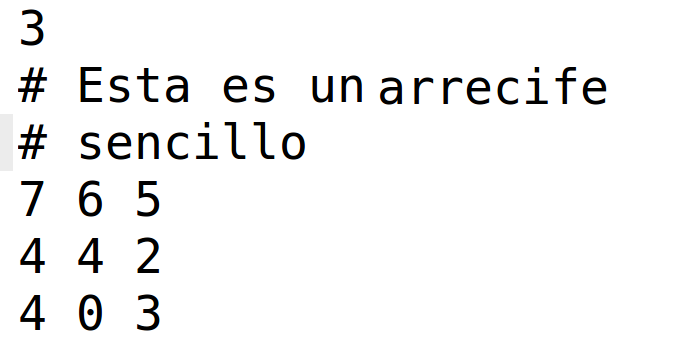
\includegraphics[width=0.25\textwidth]{entrada.png}
	\caption{Entrada simple 3x3}
	\label{fig:entrada}
\end{figure}

Con la finalidad de hacer r\'apida la ejecuci\'on de la aplicaci\'on un archivo es le\'ido una sola vez y en esta lectura se construyen colecciones para cada uno de los elementos del arrecife, una colecci\'on de coordenadas donde se ubican los tiburones, una colecci\'on de coordenadas donde se ubican los obst\'aculos o rocas, etc.

El escenario que se encuentra en memoria puede ser le\'ido por diversos algoritmos, dado que estos obtienen la posici\'on del robot y a partir de este recorre y construye \textit{el grafo}.\\

\textbf{Nemo3} Permite entradas que van desde el 2x2 hasta 20x20, aunque la ejecuci\'on de los algoritmos, tardan mucho tiempo entre mayor sea el escenario y menor cantidad de elementos (Tiburones, Rocas, Tortugas, Hombres con arp\'on y Metas) posea. Un ejemplo de esta situaci\'on es la que indica en las Figuras \ref{fig:areas} una exploraci\'on en las primeras dos figuras podr\'ia costar lo mismo, mientras una exploraci\'on en la gr\'afica podr\'ia tardar un poco mas, claro que esto depende tambi\'en de la estrategia y de condiciones de procesamiento y memoria de sistema en que se ejecuten.
\begin{figure}[!h]
	\centering
	\subfloat[Entrada 8x8 con 64 espacios disponibles]{{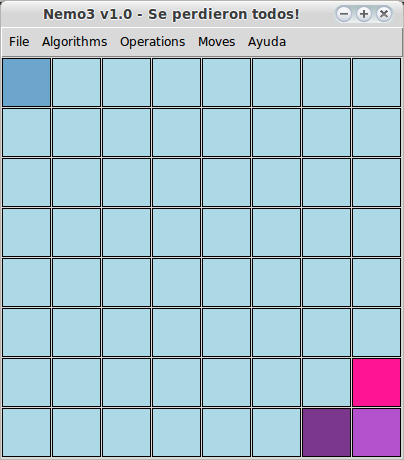
\includegraphics[width=0.2\textwidth]{en8x8.png}}}%
%	\caption{}
	\qquad
	\subfloat[Entrada 12x12 con 64 espacios disponibles]{{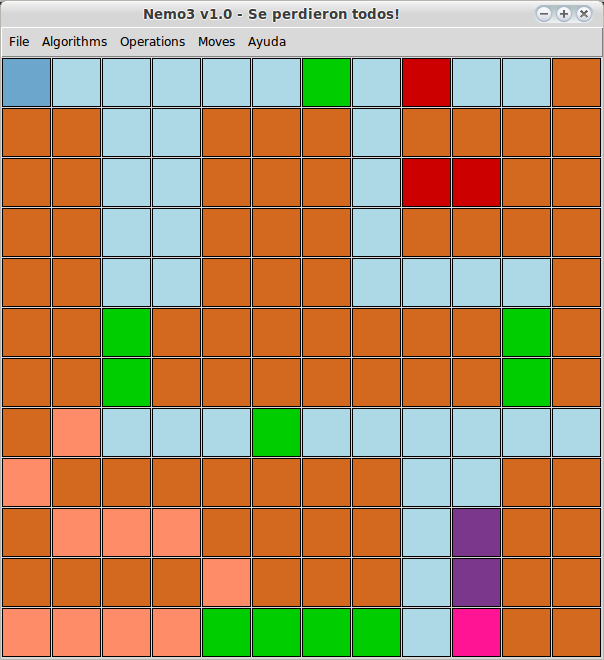
\includegraphics[width=0.2\textwidth]{en10x10.png}}}%
%	\caption{}
%	\qquad
%	\subfloat[entrada 2x2 con tres soluciones]{{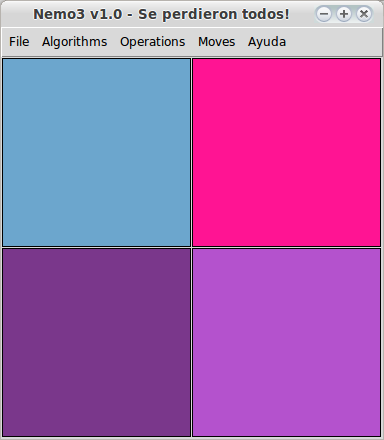
\includegraphics[width=0.1\textwidth]{en2x2.png}}}%
%	\caption{En las primeras dos gr\a'aficas el tiempo y la amplitud para un mismo algoritmo podr\'ia tardar lo mismo por el tama\~no de la exploraci\'on.\\En la entrada 2x2 la exploraci\'on deber\'ia ser menor}
	\label{fig:areas}
\end{figure}

Esto sera ampliado en la discusi\'on y el an\'alisis de los resultados. Algunas de las pruebas de entrada fueron creadas a partir de un generador ASCII en linea, con diversas dimensiones.
\section{PyNEMO 3: Aplicaci\'on con algoritmos de busqueda.}

\textbf{PyNemo 3} es una aplicaci\'on escrita en Python \cite{wiki:python} como se muestra en la Figura \ref{fig:gui} que permite cargar un archivo de texto que contiene un escenario desde un archivo de texto plano con un formato como el que se especifica en la anterior secci\'on.
\begin{figure}[!h]
	\centering
	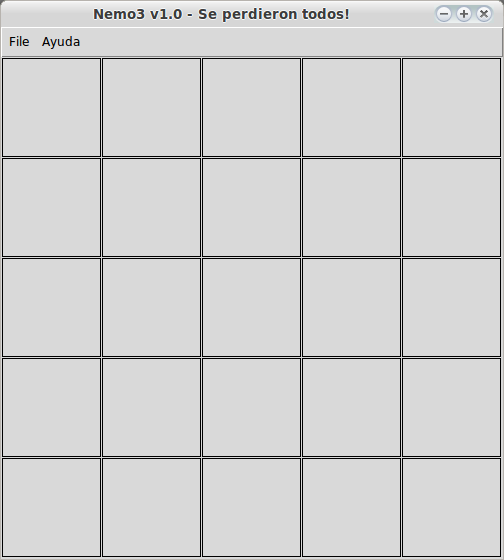
\includegraphics[width=0.3\textwidth]{gui.png}
	\caption{Interfaz grafica (GUI) de Nemo3}
	\label{fig:gui}
\end{figure}

Una vez cargado un archivo de texto este pinta un ambiente con colores que representan cada uno de los elementos especificados en el archivo y que representan el escenario de ejecuci\'on, para la entrada especificada en la \ref{fig:entrada} la interfaz gr\'afica quedara como \ref{fig:entradagui}
\begin{figure}[!h]
	\centering
	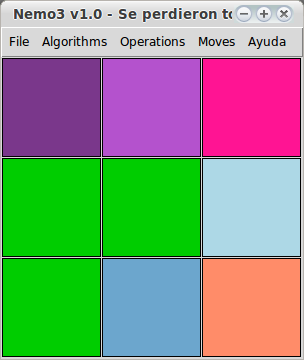
\includegraphics[width=0.3\textwidth]{entradagui.png}
	\caption{Interfaz grafica (GUI) de Nemo3}
	\label{fig:entradagui}
\end{figure}

La representaci\'on de colores que utiliza \textbf{PyNemo 3} se encuentra en un cuadro de dialogo que puede ser abierto desde el men\'u ayuda \ref{fig:ayuda}
\begin{figure}[!h]
	\centering
	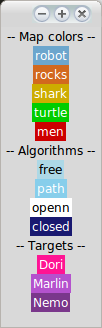
\includegraphics[width=0.1\textwidth]{ayuda.png}
	\caption{Ayuda de la Interfaz grafica (GUI) de Nemo3}
	\label{fig:ayuda}
\end{figure}

Este men\'u de ayuda indica los colores que se encuentran en el mapa, los elementos que puede modificarse con el algoritmo y los objetivos.
Esta aplicaci\'on es orientada a objetos, y por tal raz\'on un algoritmo se trata como una instancia en un hilo que puede ser detenida, ralentizada o acelerada durante la ejecuci\'on, cada uno de los algoritmos implementados, puede leer ambiente, que posee varias colecciones de acuerdo a lo que se ha encontrado en el archivo de texto.

De acuerdo con lo anterior \textbf{PyNemo 3} permite seleccionar la estrategia que el usuario final desea ejecutar en el ambiente cargado, el orden de los movimientos que desea que el algoritmo tenga en cuenta (operadores), adem\'as un conjunto de operaciones como iniciar la ejecuci\'on, detener la ejecuci\'on, hacer la transici\'on de estados, abiertos y cerrados lento o r\'apido y limpiar los cambios que ha hecho el algoritmo en la interfaz.

Una vez termine la ejecuci\'on del algoritmo se pinta la ruta que ha encontrado, además permite guardar en un archivo de texto la salida de la ejecuci\'on.\\\\
\textbf{Pasos soluc\'ion:} \( (X,Y)->(X,Y)->...->(X,Y) \)\\
\textbf{Nodos expandidos:} X \\
\textbf{Nodos creados:} Y \\
\textbf{Costo total soluci\'on:} Z \\
\textbf{Factor ramificaci\'on:} W 

La puesta en marcha realiza con el comando \textit{python nemo3.py}, la interfaz esta construida con Tkinter y con python2.7 que deben estar instalados en el computador que se desea ejecutar la aplicaci\'on

\input{resultados}
\input{conclusion}

\bibliographystyle{abbrv}
\balance
\bibliography{bibliography}
%\fixmedp{15pp limit, all inclusive}

\end{document}

